%----------------------------------------------------------------------------------------
%	PACKAGES AND THEMES
%----------------------------------------------------------------------------------------
\documentclass[aspectratio=169,xcolor=dvipsnames]{beamer}
\usetheme{SimplePlus}

\usepackage{hyperref}
\usepackage{graphicx} % Allows including images
\graphicspath{ {../output/} }
\usepackage{booktabs} % Allows the use of \toprule, \midrule and \bottomrule in tables

\usepackage{pgf-pie} % Allows creating pie charts

	
\usepackage{color, colortbl}


\usepackage{pgfplots} % Allows creating other plots
\pgfplotsset{compat=1.18}

\usepackage{caption}

\usepackage{pifont}

\usepackage{tikz} % Flow chart
\usetikzlibrary{shapes.geometric, arrows}
%----------------------------------------------------------------------------------------
%	TITLE PAGE
%----------------------------------------------------------------------------------------

\title[short title]{Heart Failure: predicting hospital re-admission after 6 months} % The short title appears at the bottom of every slide, the full title is only on the title page
\subtitle{Statistical Learning for Healthcare Data (056867) -- A.Y. 2022/2023}

\author[]{Teo Bucci, Giulia Montani and Alice Traversa}

\institute[NTU] % Your institution as it will appear on the bottom of every slide, may be shorthand to save space
{
    Politecnico di Milano% Your institution for the title page
}
\date{June 6, 2023} % Date, can be changed to a custom date


%----------------------------------------------------------------------------------------
%	PRESENTATION SLIDES
%----------------------------------------------------------------------------------------

\begin{document}

\begin{frame}
    % Print the title page as the first slide
    \titlepage
\end{frame}

\begin{frame}{Overview}
    % Throughout your presentation, if you choose to use \section{} and \subsection{} commands, these will automatically be printed on this slide as an overview of your presentation
    \tableofcontents
\end{frame}


% 10 minuti

% 1 - intro
% 2 - presentazione dei dati + data cleaning iniziale [*]
% 3 - NaN
% 4 - NaN + imputation
% 5 - outlier
% 6 - feature selection (variance based + correlation)
% 7 - Training conditions: Class imbalance, The CV approach was a StratifiedKFold with 5 folds, performance index AUC
% 8 - [RESULTS] TABLE 1 Interpretability vs complexity
% 9 - Random Forest TABLE 2 confusion matrix + performance (F1 recall, precision...)
% 10 - Explaining predictions with SHAP
% 11 - Logistic Regression: si allena velocemente, quindi feature selection scegliendo un numero di features guardando l'AUC al diminuire delle features
% 13 - limitations, further development and recommendations
% 
% 
% 
% [*] The majority of patients had age in the 59-89
% range, namely a total of 1680 patients accounting
% for 86.11% of the total. Regarding sex, 58.18% were
% females and 41.82% were males.
% 73.50% suffered a whole HF, while 23.89% suf-
% fered a Left HF and 2.61% a Right HF




%------------------------------------------------
\section{Introduction}
%------------------------------------------------



\begin{frame}{Problem statement}
    Heart failure (HF) is a prevalent condition with high re-admission rates.\\
    Number of HF cases worldwide:
    \begin{itemize}
        \item 33.5 million in 1990;
        \item 64.3 million in 2017.
    \end{itemize}
    
    Patients diagnosed with HF will be re-admitted once within a year and 20\% will be re-admitted twice or more.

    \begin{block}{Goal of the project}
        Develop a prediction model with focus on interpretability.
    \end{block}

\end{frame}



%------------------------------------------------
\section{Materials and methods}
%------------------------------------------------

%------------------------------------------------

\begin{frame}{Data Overview}
    \begin{columns}[c]
        \column{.6\textwidth}
        \begin{itemize}
            \item 2008 patients admitted to a hospital
            \item 168 variables provided, including:
            \begin{enumerate}
                \item Demographic data (height, sex, occupation, \ldots).
                \item Medical history (diabetes, comorbidities, \ldots).
                \item Clinical measurements (pressure, hemoglobyn, \ldots).
                \item Drugs taken.
            \end{enumerate}
        \end{itemize}
        \begin{alertblock}{Inconsistencies}
            57 dead patients and all information on re-hospitalizations prior to 6 months are removed
        \end{alertblock}

        \column{.4\textwidth}
        \begin{figure}
            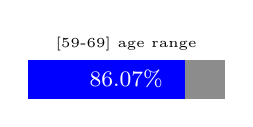
\begin{tikzpicture}
                \fill[Blue] (0,0) rectangle (2.5,0.5);
                \fill[Gray!90] (2.5,0) rectangle (2,0.5);
                \node at (1.25,0.25) [align=center] {\footnotesize \color{white}86.07\%};
                \node at (1.25,0.7) {\tiny [59-69] age range};
            \end{tikzpicture}
        \end{figure}

        \begin{figure}
            \resizebox{0.6\textwidth}{!}{
            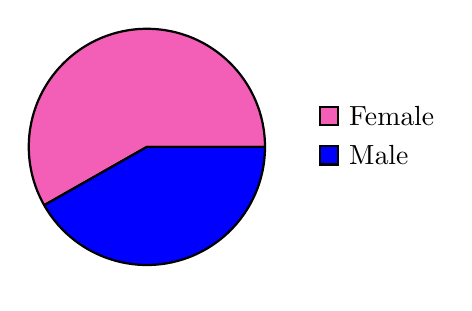
\begin{tikzpicture}
                \pie[
                    color={CarnationPink, Blue},
                    sum=auto,
                    text=legend,
                    before number=\phantom,,
                    radius=1.5
                ]{
                    58.22/Female,
                    41.78/Male
                }
            \end{tikzpicture}
            }
            %\caption{Distribution of Sex.}
        \end{figure}

        \begin{figure}
            \resizebox{0.6\textwidth}{!}{
            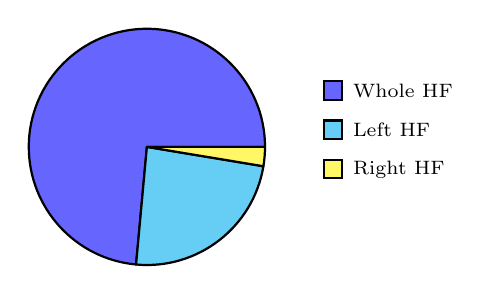
\begin{tikzpicture}[font=\scriptsize]
                \pie[
                    sum=auto,
                    text=legend,
                    before number=\phantom,,
                    radius=1.5
                ]{
                    73.54/Whole HF,
                    23.84/Left HF,
                    2.62/Right HF
                }
            \end{tikzpicture}
            }
            %\caption{Distribution of Heart Failure types.}
        \end{figure}

    \end{columns}
\end{frame}

%------------------------------------------------

\begin{frame}{Handling missing values}

    \begin{columns}[t]
        \column{.45\textwidth}
        \textbf{Numerical features}

        \begin{itemize}
            \item 14 features with over 60\% missing are discarded
            \item 9 features between 50\% and 60\% are discarded after further analysis
            \item Imputation: KNN with 5 neighbors 
        \end{itemize}

        \vspace{0.5cm}
        
        \textbf{Categorical features}
        
        \begin{itemize}
            \item \texttt{Occupation} 1.34\%
            \item Imputation: most frequent
        \end{itemize}

        \column{.55\textwidth} 
        \begin{figure}[htpb]
            \centering
            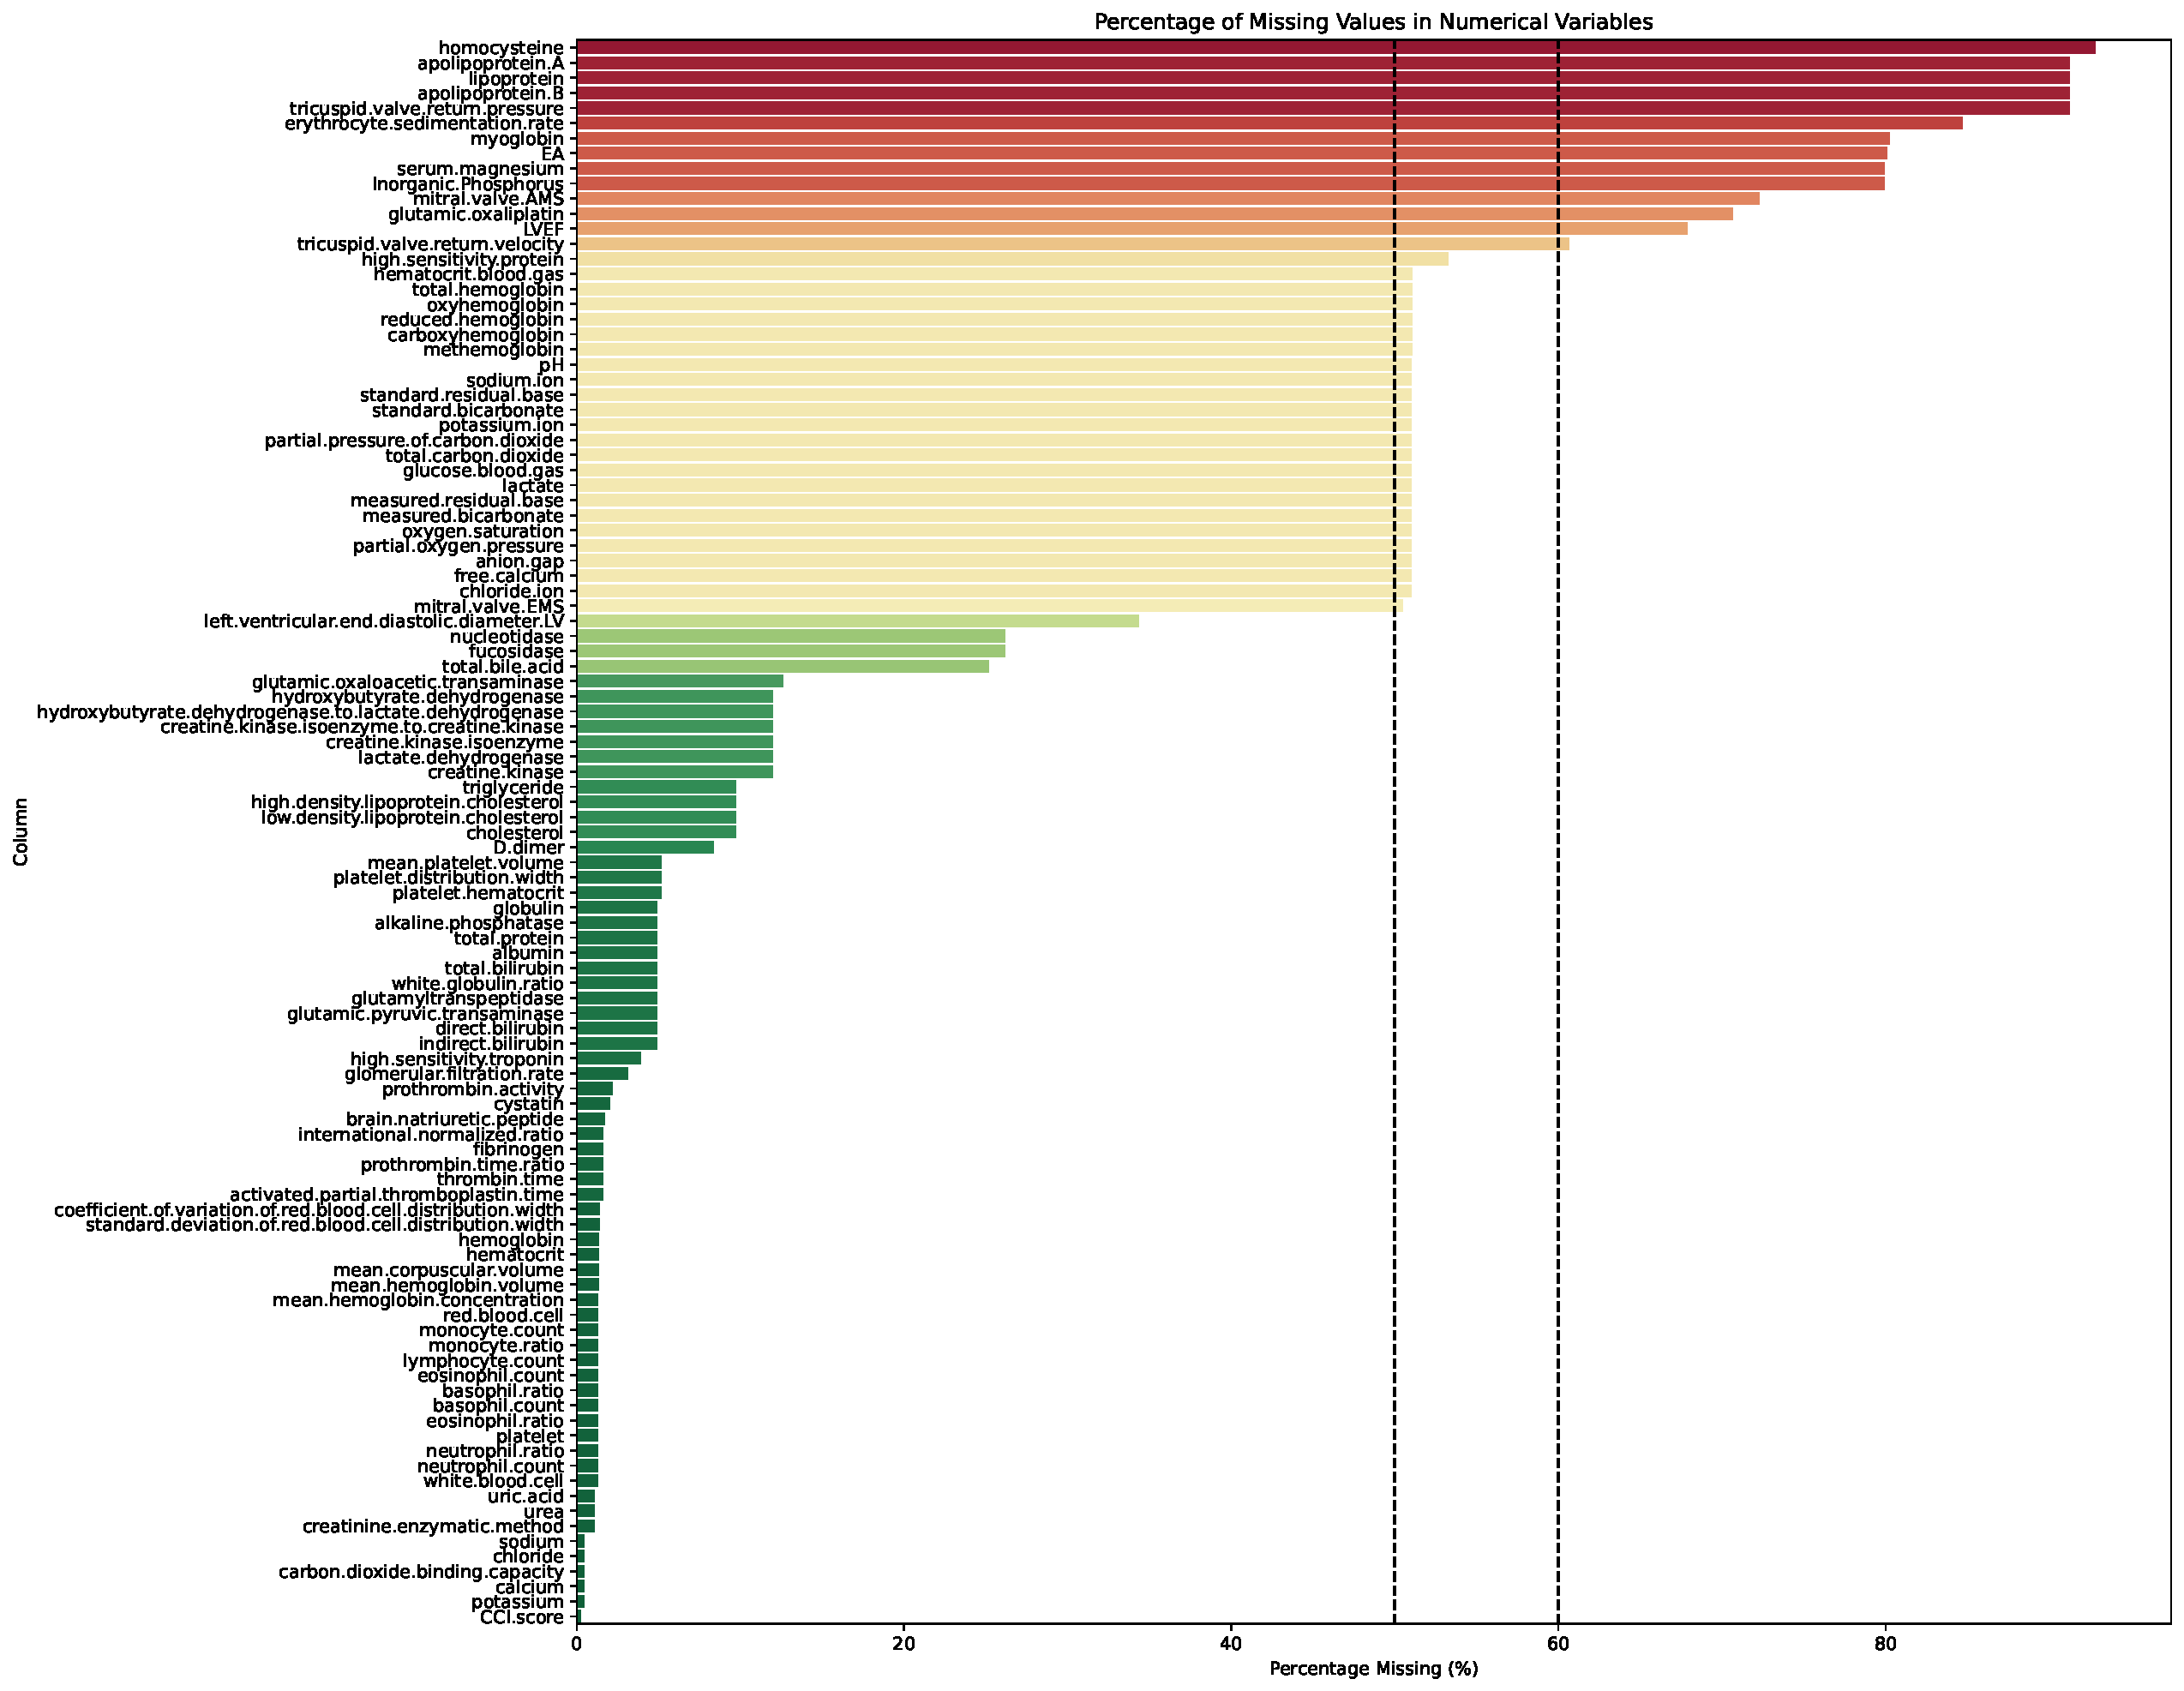
\includegraphics[width=0.9\textwidth]{missing_values_percentages.pdf}
            \captionsetup{font=tiny} % Set the caption font size to small
            \caption{Percentage of missing values in numeric.}
        \end{figure}
        
    \end{columns}

\end{frame}

%------------------------------------------------

\begin{frame}{Pruning variables}
\begin{itemize}
    \item \textbf{Outlier analysis}
    \begin{enumerate}
        \item Identification:
            \begin{itemize}
                \item Sample Z-scores
                \item Physiological possibility of outlier values checked using literature.
            \end{itemize}
        \item Replace with \text{NaN} for imputation.
    \end{enumerate}

    \item \textbf{Low variance variable:}
    Remove \alert{16} variables with more than \alert{95\% dominance}

    \item \textbf{Correlation analysis:}
    Remove \alert{12} variables with more than \alert{85\% correlation}
\end{itemize}

Three variables with possible outliers retained due to their importance:
\begin{itemize}
    \item \texttt{eosinophil.count}
    \item \texttt{high.sensitivity.troponin}
    \item \texttt{glutamic.pyruvic.transaminase}
\end{itemize}

\end{frame}
%------------------------------------------------
\tikzstyle{method1} = [rectangle, rounded corners, 
minimum width=4cm, 
minimum height=1cm,
text width=4cm,
text centered, 
draw=black, 
fill=CornflowerBlue]

\tikzstyle{method2} = [rectangle, rounded corners, 
minimum width=4cm, 
minimum height=1cm,
text width=4cm,
text centered, 
draw=black, 
fill=Peach]

\tikzstyle{union1} = [rectangle, 
minimum width=1cm, 
minimum height = 0.5cm,
text centered, 
draw=black]

\tikzstyle{union2} = [rectangle, 
minimum width=1cm, 
minimum height = 0.5cm,
text centered, 
draw=Red]

\begin{frame}{Feature selection}

    \begin{figure}[!h]
    \centering
        \begin{tikzpicture}[node distance=2cm]
            \node (RF) [method1] {Random Forest
            \tiny{Set of 30 features : $S_{RF}$}};
            \node (LR) [method1, below of=RF] {Logistic Regression
            \tiny{Strong $L^{1}$ penalty : $S_{LR}$}};
            \node (U1) [union1, right of = LR, yshift= 1cm, xshift = 1cm] {\tiny{$S_{RF}\cup S_{LR}$}};
            \node (BS) [method2, right of = U1, yshift = 1cm, xshift = 1cm] {Backward
            \\ \tiny{Based on AUC evolution : $S^{\star}_{1}$}};
            \node (FS) [method2, right of = U1, yshift = -1cm, xshift = 1cm] {Forward 
            \\ \tiny{Select 10 : $S^{\star}_{2}$ }};
            \node (U2) [union2, right of = FS, yshift= 1cm, xshift = 2cm] {\tiny{$S = S^{\star}_{1}\cup S^{\star}_{2}$}};
    
            \draw [->] (RF) -- (U1);
            \draw [->] (LR) -- (U1);
            \draw [->] (U1) -- (BS);
            \draw [->] (U1) -- (FS);
            \draw [->] (FS) -- (U2);
            \draw [->] (BS) -- (U2);
            
        \end{tikzpicture}
    \end{figure}

    %\vspace{5cm}
    
    %\textbf{Strength of the method:} 
    %\begin{itemize}
    %    \item Faster than backward selection
    %    \item Take advantages of both RF and LR
    %    \item Final set of 13 selected variables.
    %\end{itemize}

    \begin{block}{Strength of the method}
    \begin{itemize}
        \item Faster than backward selection
        \item Take advantages of both RF and LR
        \item Final set of 13 selected variables.
    \end{itemize}
    \end{block}

    
\end{frame}

%------------------------------------------------
\begin{frame}{Modelling choice}

\textbf{Metric}
\begin{itemize}
    \item Area Under Curve (AUC) under the Receiver Operating Characteristic (ROC) curve.
\end{itemize}
\textbf{Training setting} 
\begin{itemize}
    \item Stratified 5-fold cross-validation (CV).
    \item 85:15 stratified train-test ratio.
    \item Seed always set for reproducibility.
    \item Class imbalance: \alert{39.6\%} of observations belonging to class 1, addressed by passing class weights based on sample proportions.
\end{itemize}
    
\end{frame}


%------------------------------------------------
\section{Results}
%------------------------------------------------



%------------------------------------------------

\begin{frame}{Results}

    \begin{columns}[c]
        \column{.5\textwidth}
        \begin{table}[htpb]
        \centering
        %\caption{Comparison of performance.}
        \label{tab:performance}
        \begin{tabular}{lr}
        \toprule
                         Model &    AUC \\
        \midrule
        RandomForestClassifier & 0.6769 \\
        \rowcolor{green!50}
            LogisticRegression & 0.6702 \\
                    GaussianNB & 0.6452 \\
        DecisionTreeClassifier & 0.5943 \\
          KNeighborsClassifier & 0.5681 \\
                 MLPClassifier & 0.5028 \\
        \bottomrule
        \end{tabular}
        \caption{Comparison of performance.}
        \end{table}

        \column{.5\textwidth}
        \begin{figure}[htpb]
            \centering
            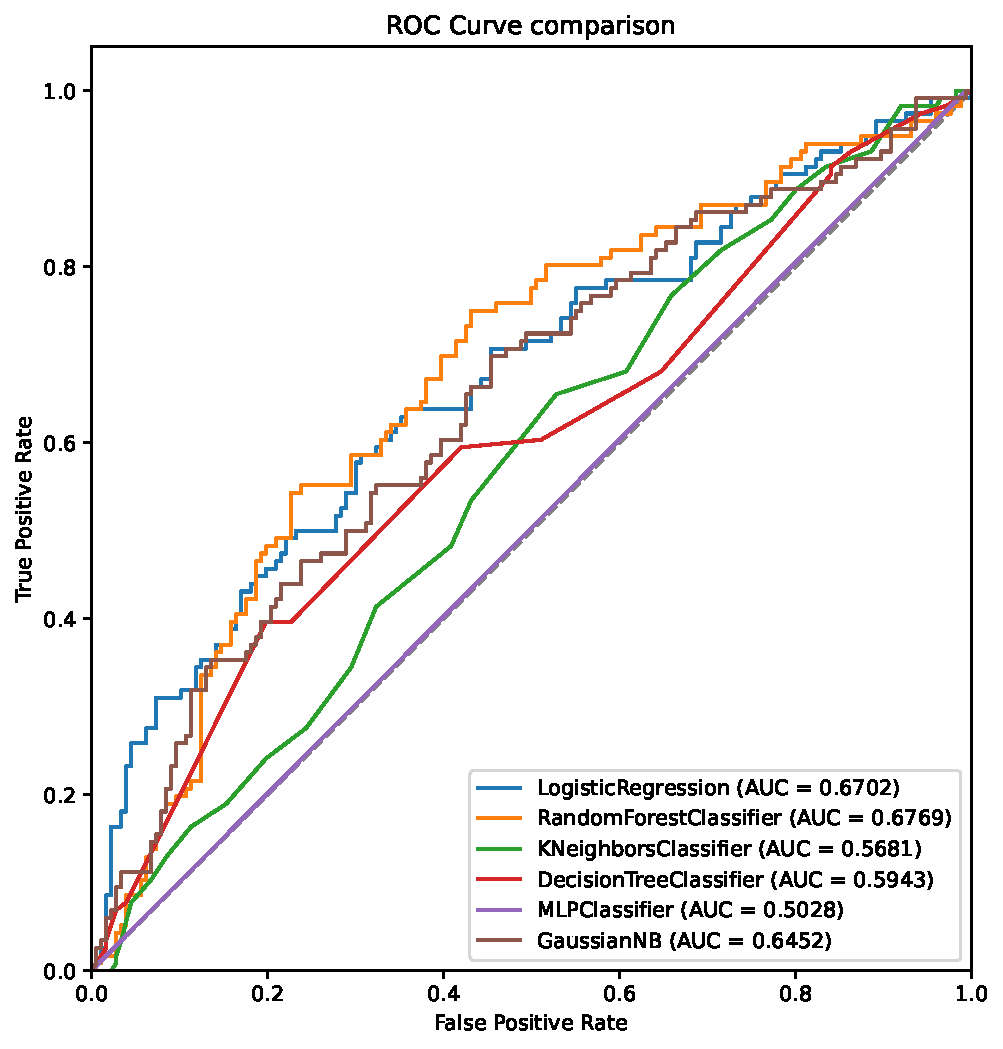
\includegraphics[width=2.1in]{roc_comparison.pdf}
            \caption{ROC curves comparison.}
            \label{fig:roc-comparison}
        \end{figure}
    \end{columns}

\end{frame}




%------------------------------------------------

\begin{frame}{Performance evaluation}

    \begin{columns}[c]

        \column{.5\textwidth} 
        \begin{figure}[htpb]
            \centering
            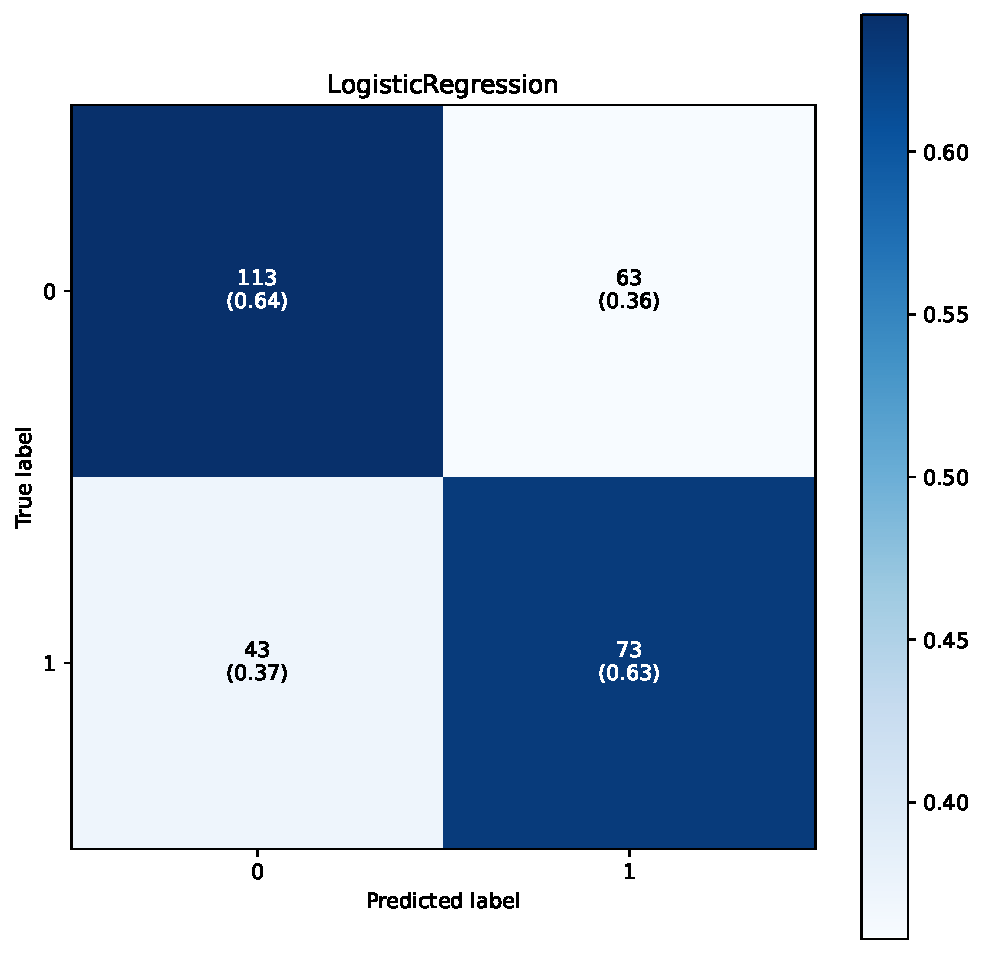
\includegraphics[width=1.6in]{confusion_matrix_LR.pdf}
            \caption{Normalized confusion matrix of the LR.}
            \label{fig:confusion}
        \end{figure}

        \column{.5\textwidth}
        \centering
        \begin{table}
            \resizebox{0.8\textwidth}{!}{
            \begin{tabular}{lrrrr}
            \toprule
            {} &  precision &  recall &  f1-score &  support \\
            \midrule
            False        &     0.7244 &  0.6420 &    0.6807 &      176 \\
            True         &     \textbf{0.5368} &  \textbf{0.6293} &    \textbf{0.5794} &      116 \\
            macro avg    &     0.6306 &  0.6357 &    0.6300 &      292 \\
            weighted avg &     0.6498 &  0.6370 &    0.6405 &      292 \\
            \bottomrule
            \end{tabular}
            }
            \caption{Classification report.}
        \end{table}
        Accuracy: 0.6370
        
    \end{columns}

    \vspace{0.5cm}
    Deployment in a \textbf{web app} for easy usage:\\
    \url{https://teobucci-slhd-app-3iahgf.streamlit.app/}

\end{frame}


%------------------------------------------------
\section{Discussion and conclusion}
%------------------------------------------------


%------------------------------------------------
\begin{frame}{Discussion and conclusion}

    \begin{columns}[c]

        \column{.5\textwidth}
        %\centering
        %\begin{figure}[htpb]
        %    \centering
        %    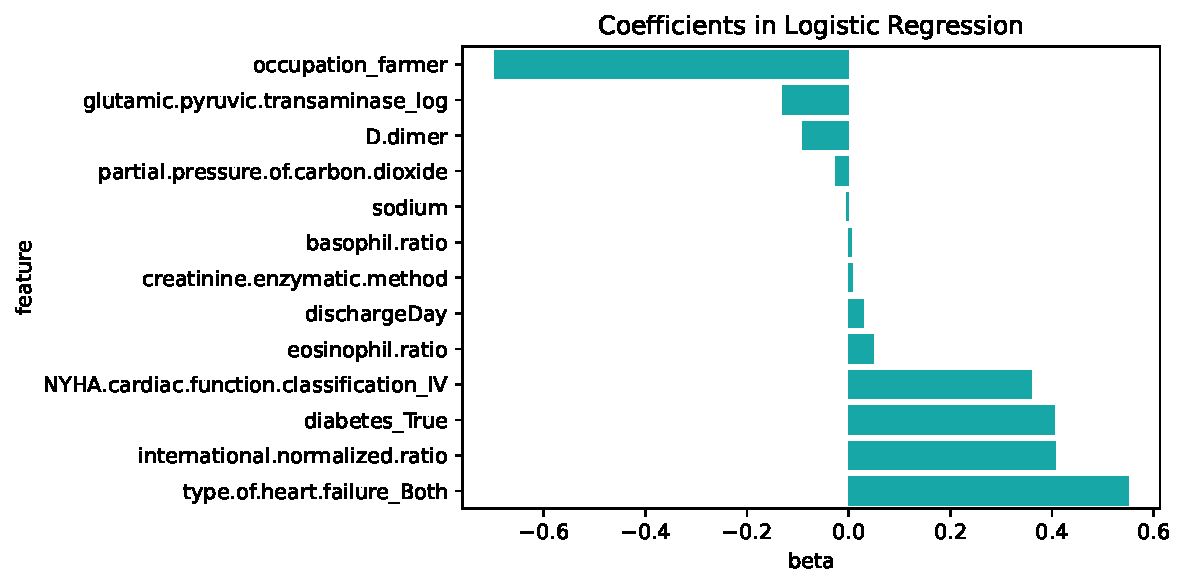
\includegraphics[width=2.6in]{feature_importance_weightsLogisticRegression.pdf}
        %    %\caption{Coefficients of the \gls{lr}.}
        %    \label{fig:feature-importance-logistic-regression}
        %\end{figure}

        \begin{table}[h!]
            \centering
        \resizebox{\textwidth}{!}{
        \begin{tabular}{lrr}
            \toprule
                                            feature &    beta &  exp\_beta \\
            \midrule
\rowcolor{green!50}
                                  occupation\_farmer & -0.6973 &    0.4979 \\
                  glutamic.pyruvic.transaminase\_log & -0.1305 &    0.8776 \\
\rowcolor{green!50}
                                            D.dimer & -0.0911 &    0.9129 \\
                 partial.pressure.of.carbon.dioxide & -0.0261 &    0.9743 \\
                                             sodium & -0.0049 &    0.9951 \\
                                     basophil.ratio &  0.0055 &    1.0055 \\
                        creatinine.enzymatic.method &  0.0066 &    1.0066 \\
\rowcolor{red!50}
                                       dischargeDay &  0.0294 &    1.0298 \\
                                   eosinophil.ratio &  0.0486 &    1.0498 \\
\rowcolor{red!50}
            NYHA.cardiac.function.classification\_IV &  0.3599 &    1.4332 \\
\rowcolor{red!50}
                                      diabetes\_True &  0.4049 &    1.4991 \\
                     international.normalized.ratio &  0.4074 &    1.5029 \\
\rowcolor{red!50}
                         type.of.heart.failure\_Both &  0.5502 &    1.7336 \\
            \bottomrule
            \end{tabular}
        }
            \caption{LR coefficients.}
            \label{tab:my_label}
        \end{table}



        \column{.5\textwidth}
        \centering
        \begin{itemize}
            \item Farmers are less likely to be re-admitted (probably external confounder).
            \item D-dimer seems associated with tissue repair.
            \item Higher discharge day (i.e. longer stay in hospital) is associated with higher risk.
            \item Level 4 NYHA, presence of diabetes and having suffered a Whole HF highly associated with re-admission.
        \end{itemize}
    \end{columns}
    
\end{frame}





% \begin{frame}{Limitations and Recommendations}
% \begin{itemize}
%   \item Limitations: reliance on \textbf{single dataset} and difficulty in \textbf{comparing results}, sample is \textbf{not representative}, missing data imputation, lacking data coming from electrocardiography.
%   \item Recommendations: better \textbf{management of missing values}, further validation with \textbf{external datasets}, exploration of \textbf{additional predictive models}.
% \end{itemize}
% \end{frame}
\begin{frame}{Limitations and Recommendations}
\textbf{Limitations}
\begin{itemize}
  \item reliance on \textbf{single dataset}
  \item difficulty in \textbf{comparing results}
  \item the sample is \textbf{not representative}
  \item missing data imputation
  \item lacking data coming from electrocardiography.
\end{itemize}

\textbf{Recommendations}
\begin{itemize}
  \item better \textbf{management of missing values}
  \item further validation with \textbf{external datasets}
  \item exploration of \textbf{additional predictive models}.
\end{itemize}
\end{frame}






% \begin{frame}[fragile] % Need to use the fragile option when verbatim is used in the slide
%     \frametitle{Citation}
%     An example of the \verb|\cite| command to cite within the presentation:\\~

%     This statement requires citation \cite{p1}.
% \end{frame}

% %------------------------------------------------

% \begin{frame}{References}
%     % Beamer does not support BibTeX so references must be inserted manually as below
%     \footnotesize{
%         \begin{thebibliography}{99}
%             \bibitem[Smith, 2012]{p1} John Smith (2012)
%             \newblock Title of the publication
%             \newblock \emph{Journal Name} 12(3), 45 -- 678.
%         \end{thebibliography}
%     }
% \end{frame}

%------------------------------------------------

\begin{frame}
    \Huge{\centerline{\textbf{Thank You!}}}
\end{frame}

%----------------------------------------------------------------------------------------

\end{document}